% !TEX root = ../../vzor.tex
%% Ukázka: TikZ: geometrický nákres, vývojový diagram
%% Vkládá ji soubor vzor/kapitoly/prakticka.tex; ve vzor.pdf je pod nadpisem uvedeno „Zdroj ukázky".
%% Vyžaduje balíček tikz – v mprace.tex odkomentujte připravený řádek s \usepackage.

\section{Diagramy v prostředí TikZ}
\zdrojukazky{vzor/ukazky/tikz.tex}

Balíček \texttt{tikz} je v šabloně volitelný: v souboru \texttt{mprace.tex}
odkomentujte řádek s \verb|\usepackage{tikz}|.

Prostředí \texttt{tikzpicture} umožňuje kreslit vektorové diagramy přímo v \LaTeX{}u.

\textbf{Geometrický nákres} – pravoúhlý trojúhelník:
\begin{center}
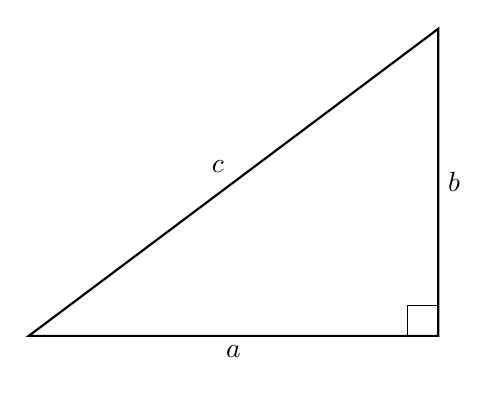
\begin{tikzpicture}[scale=1.3]
	\draw[thick] (0,0) -- (4,0) -- (4,3) -- cycle;
	\draw (3.7,0) -- (3.7,0.3) -- (4,0.3);		% pravý úhel
	\node[below] at (2,0) {$a$};
	\node[right] at (4,1.5) {$b$};
	\node[above left] at (2,1.5) {$c$};
\end{tikzpicture}
\end{center}

\textbf{Vývojový diagram} – jednoduchý flowchart:
\begin{center}
\begin{tikzpicture}[
	node distance=1.4cm,
	box/.style={rectangle, draw, rounded corners, minimum width=3cm,
	            minimum height=0.7cm, text centered},
	dec/.style={diamond, draw, minimum width=3cm, minimum height=0.7cm,
	            text centered, aspect=2.5}
]
	\node[box] (start) {Start};
	\node[box, below=of start] (vstup) {Vstup: $n$};
	\node[dec, below=of vstup] (podm) {$n > 0$\,?};
	\node[box, below=of podm] (vypis) {Vypiš $n$};
	\node[box, below=of vypis] (end) {Konec};
	\draw[->] (start) -- (vstup);
	\draw[->] (vstup) -- (podm);
	\draw[->] (podm) -- node[right] {ano} (vypis);
	\draw[->] (vypis) -- (end);
	\draw[->] (podm.east) -- node[above] {ne} ++(2.2,0) |- (end.east);
\end{tikzpicture}
\end{center}
